\documentclass[10pt,a4paper]{article}
\usepackage[margin=0.8in]{geometry}
\usepackage[T1]{fontenc}
\usepackage[utf8]{inputenc}
\usepackage{lmodern,amsmath,amssymb,booktabs,array,enumitem}
\usepackage[expansion=false]{microtype}
\usepackage{csquotes}
\usepackage{xurl,hyperref,tabularx,graphicx,xcolor}
\usepackage[section]{placeins}
\hypersetup{hidelinks}
\newcolumntype{Y}{>{\raggedright\arraybackslash}X}
\newcolumntype{L}[1]{>{\raggedright\arraybackslash}p{#1}}
\setlength{\parindent}{0pt}
\setlength{\parskip}{4pt}
\setlength{\tabcolsep}{3pt}
\renewcommand{\arraystretch}{1.12}
\setlist{nosep,leftmargin=*}
\newcommand{\figw}{\linewidth}

\title{\textbf{Computer Networks --- Research Project}\\[4pt]
\large Phase 3: Implementation, Experiments and Results\\[8pt]
\Large Poisoning, Retention and Legitimate Adaptation\\in Federated Continual Intrusion Detection}
\author{Saneedullah (23I-2568) \qquad Ahmed Bilal (23I-2581)}
\date{November 2026}

\begin{document}
\maketitle

\begin{abstract}
Intrusion detection systems must learn new attack families without forgetting old ones, and are increasingly trained federally. Phase 2 identified an untested combination: label poisoning that happens \emph{while} a federated continual learner acquires a new attack family, and defences that may discard legitimate new evidence together with the poison. Phase 3 implements the Phase 2 design in our own code and runs it on the corrected CICIDS2017 benchmark: five clients, four attack-family stages, three learners (fine-tuning FT, an EWC-style regulariser EI, DER++ replay DR), three admission rules (class-aware DC, matched global DM, random class-aware DQ), and six attack arms (one, three or five attacking clients, 25--90\% of the Hulk rows relabelled benign in stage two). We ran 696 experiments, grouped into 12 paired units (three ownership partitions $\times$ four training replicates), on the development bank only. Replay is the only learner that retains earlier families (clean macro-F1 0.49 against 0.03--0.05), but it also keeps poisoned knowledge: after the attacker withdraws, DR still loses 0.79 of its Hulk recall at 50\% poisoning and 0.99 at 90\%. A single attacker among five clients is largely diluted by federated averaging. None of the tested admission rules reduced persistent damage. The class-aware quota kept all new-class rows where the global filter kept 9.5\% under the strongest attack, but ranking by loss inside the quota cost acquisition and macro-F1. Ablations show that the replay-label term and the memory eviction rule decide both retention and how much poison survives. We do not claim better accuracy than prior work; the contribution is evidence on a combination that earlier studies did not test.
\end{abstract}
\noindent\textbf{Keywords:} continual learning; federated learning; intrusion detection; label poisoning; replay memory; admission control.

%=====================================================================
\section{Introduction and Scope}
Phase 1 reviewed three 2026 studies of continual learning for network security \cite{ge,wu,luo}. Phase 2 extended the review with ten further 2025--2026 studies (P4--P13) and narrowed three gaps into three research questions \cite{phase1}:
\begin{itemize}
\item \textbf{RQ1} (gap G1): How do fine-tuning, an EWC-style regulariser and DER++ replay differ in the damage a poisoned stage causes to the targeted attack family, both immediately and after the attacker withdraws?
\item \textbf{RQ2} (gap G2): Compared with a global filter that admits the same number of samples, how does a class-aware admission rule change the trade-off between poisoning damage and the learning of new attack families?
\item \textbf{RQ3} (gap G3): Which memory and selection mechanisms explain the differences, and what do they cost in computation and communication?
\end{itemize}
This report covers the seven Phase 3 requirements: the implementation (Section~\ref{sec:impl}), dataset and preprocessing (Section~\ref{sec:data}), baseline evaluation (Section~\ref{sec:base}), graphical results (Sections~\ref{sec:base}--\ref{sec:def}), ablation studies (Section~\ref{sec:abl}), comparison with existing research (Section~\ref{sec:lit}), and the analysis and discussion of the results (Section~\ref{sec:disc}).

\subsection{What changed from the Phase 2 plan}
We report every deviation, with its reason.
\begin{itemize}
\item \textbf{Attack strength (pre-declared fallback).} Phase 2 stated that if a single attacker had no visible effect, a fallback would be tried and, failing that, the dilution by federated averaging would be reported as a finding. Our first complete run (three seeds, one attacker, up to the full set of that client's Hulk rows) showed exactly this: the attacker held about 6\% of the Hulk rows of the first partition, and Hulk recall stayed at 0.99--1.00 with an attack success rate of 0. We therefore extended the threat model to one, three or five attacking clients and to partial doses (Table~\ref{tab:grid}). The strongest arm uses a dose of 0.9, not 1.0, because with five attackers and dose 1.0 no Hulk label survives and the class would never receive an output unit.
\item \textbf{Seeds.} Phase 2 planned twelve seeds. The repository allows only the development seeds 101--103 and seals higher seeds for the final evaluation, which we did not run. We therefore use three ownership partitions (101--103) $\times$ four training replicates = 12 paired units. Replicates inside one partition share their client ownership and are not independent; confidence is therefore bounded by the three partitions.
\item \textbf{Admission conditions.} Phase 2 listed DG, DM and DC. We implemented DC, DM and a random class-aware control DQ (same quota as DC, random choice inside each class); the unmatched global filter DG was not run.
\item \textbf{Not done.} The external CICIoT2023 check, the poisoned-memory diagnostic with cloned states, inference-latency measurement, and the sealed final evaluation. Cost is reported as wall time, communicated bytes and memory bytes.
\item \textbf{Hyper-parameters.} Learner settings were taken from the repository's development-seed selection (Table~\ref{tab:hp}); we did not tune them.
\end{itemize}
All results are on the fixed development bank. No final-test data were read.

%=====================================================================
\section{Implementation of the Proposed Methodology}\label{sec:impl}
\subsection{Federation and model}
Five persistent clients learn four successive stages E1--E4 (Table~\ref{tab:classes}). Each stage consists of 12 synchronisation rounds; in every round each client trains one local epoch (Adam, learning rate $10^{-3}$, batch 256) from the current global model, and the server averages the client models with FedAvg \cite{fedavg}, weighting each client by the number of rows it admitted. The classifier is a small MLP, $74\rightarrow128\rightarrow64\rightarrow C_t$ with dropout 0.1, where the output layer grows with each stage ($C_t = 3, 8, 13, 16$ output units); growth keeps the old logits unchanged. The final model has 18,896 parameters (75.6~KB). Each class slot is created when a class first appears with a label in a client's training data. Whole network components belong to one client, so no row leaks between clients.

\subsection{Learners}
\begin{itemize}
\item \textbf{FT}: sequential fine-tuning with no retention mechanism.
\item \textbf{EI} (EWC-style \cite{ewc}): after each stage each client estimates a per-example diagonal Fisher importance on up to 1,024 of its admitted rows; the server averages them (weighted by admitted rows) and accumulates them across stages. Later training adds the penalty $\tfrac{\lambda_E}{2}\sum_i F_i(\theta_i-\theta^\ast_i)^2$ with $\lambda_E=100$ around the previous model; new output rows have zero importance.
\item \textbf{DR} (DER++ \cite{der}): each client keeps a 500-record memory filled by reservoir sampling \cite{vitter}. A record stores the input, its (possibly poisoned) label and the model's logits when it was first seen. Local training adds a replay cross-entropy term ($\lambda_y=1$) and a logit-matching term ($\lambda_z=0.1$) on a replay batch of 128.
\end{itemize}

\subsection{Poisoning model}
In stage E2 a set of $k$ attacking clients each relabel a fraction $\rho$ of their own DoS-Hulk training rows as benign. The attacking clients and the order of rows are drawn from a seeded stream; doses are nested prefixes, and the attacking sets are nested ($k{=}1\subset k{=}3\subset k{=}5$), so every comparison is paired. The attack is withdrawn in E3 and E4 (no poison and no fresh Hulk rows), so any Hulk error remaining at E4 measures persistence, not re-learning.

\subsection{Admission rules}
All rules are applied per client and per stage, with scores from the current model after head expansion. Classes that are new at the stage, or have fewer than $n_{\min}=20$ rows, are kept whole.
\begin{itemize}
\item \textbf{DC} (class-aware): inside every other class keep the fraction $q=0.75$ with the lowest loss.
\item \textbf{DM} (matched global): keep the same number of rows as DC, but chosen by global loss ranking over all rows.
\item \textbf{DQ} (control): the same per-class quota as DC, but a random choice inside each class.
\end{itemize}
All three admit exactly the same number of rows per client (verified in the code tests), so differences are not caused by volume.

\subsection{Metrics}
Stage macro-F1 on the scored classes of the fixed development bank; benign false-alarm rate (FAR); Hulk recall and attack success rate (ASR, share of Hulk rows predicted benign); immediate damage $\Delta$rec (Hulk recall lost at E2, against the same learner without attack); persistent damage $H$ (Hulk recall lost at E4, against the same learner, admission rule and setting without attack); acquisition $A$ (mean F1 of the new scored classes of stages E2--E4, Hulk excluded); backward transfer (BWT) and forgetting \cite{clmetrics}; cost (wall time, communicated bytes, model and memory bytes). The unit of analysis is one complete run; every comparison is paired by unit.

\subsection{Statistics}
We follow the Phase 2 plan: two-sided Wilcoxon signed-rank tests \cite{wilcoxon}, Holm correction inside each of two families \cite{holm}, 95\% bootstrap intervals (10,000 resamples of whole units) and the rank-biserial effect size. Family C1 compares learner pairs on $H$ and $\Delta$rec for each attacked arm (30 tests). Family C2 compares DC with DM on $A$ (six arms), on $H$ and $\Delta$rec (five attacked arms each) and on clean FAR (17 tests). All other analyses are descriptive.

\subsection{Engineering and reproducibility}
All computation ran on Kaggle (Tesla T4) in a single notebook with three parts whose outputs are saved separately: Part~A downloads the corrected dataset, rebuilds the derived data and checks every pinned file hash of the repository, and builds one training package per seed; Part~B runs the grid with our own implementation (\texttt{src/p3lib.py}), executed by four parallel worker processes (\texttt{src/p3parallel.py}), writing one result file per run and resuming after interruptions; Part~C produces all tables, figures and statistics from the saved runs. Each run is fully determined by its configuration: re-running a configuration on one device reproduces its confusion matrices exactly (tested on CPU). CPU and GPU runs are not bit-identical, so all reported runs use the GPU.

\begin{table}[htbp]
\centering\footnotesize
\caption{Settings used in all runs (adopted from the repository's development selection; not tuned here).}
\label{tab:hp}
\begin{tabularx}{\linewidth}{L{4.2cm}Y}
\toprule
Item & Value\\
\midrule
Rounds $\times$ local epochs per stage & 12 $\times$ 1\\
Optimiser, learning rate, batch & Adam, $10^{-3}$, 256\\
Model & MLP 74-128-64-$C_t$, dropout 0.1, 18,896 parameters at $C_t{=}16$\\
EI & $\lambda_E=100$, Fisher on $\le$1,024 rows per client\\
DR & memory 500 per client (reservoir), replay batch 128, $\lambda_y=1$, $\lambda_z=0.1$\\
DC / DM / DQ & $q=0.75$, $n_{\min}=20$, new classes kept whole\\
Platform & Tesla T4, PyTorch 2.11 (CUDA), four parallel workers\\
\bottomrule
\end{tabularx}
\end{table}

%=====================================================================
\section{Dataset and Preprocessing}\label{sec:data}
We use CICIDS2017 \cite{dataset} in its corrected-label release \cite{engelen}, downloaded and verified by SHA-256 (343,549,013 bytes) in the notebook. The repository's audited pipeline produces 74 header-free flow features (no addresses, ports or timestamps), a split into training pool and a fixed development bank with no overlap, and a taxonomy of 16 classes arriving over four stages (Table~\ref{tab:classes}). The benign class is capped in training (14,000 rows) while the development bank keeps all its 216,158 benign rows, so the false-alarm rate is measured on a large benign set. Classes with fewer than 50 development rows or too few independent components are not scored (Heartbleed, Infiltration and three web-attack classes) but are present in training and in the output space. Training rows total 183,045 per seed. Each of the seeds 101--103 produces its own ownership partition of whole components over the five clients; every package is checked against the taxonomy (row counts, arrival stage) before any run, and the notebook confirms that no test rows and no development rows enter a training package. Every file that the repository pins by hash matched after the rebuild.

\begin{table}[htbp]
\centering\footnotesize
\caption{Classes of the corrected CICIDS2017 benchmark: arrival stage, scoring eligibility and rows (training package of seed 101; fixed development bank).}
\label{tab:classes}
\begin{tabularx}{\linewidth}{rYcccr}
\toprule
Code & Class & Arrives & Scored & Train rows & Dev rows\\
\midrule
0 & Benign & E1 & yes & 14,000 & 216,158\\
1 & Bot & E4 & yes & 441 & 148\\
2 & DDoS & E4 & yes & 57,086 & 19,029\\
3 & DoS GoldenEye & E2 & yes & 4,540 & 1,513\\
4 & DoS Hulk & E2 & yes & 95,080 & 31,694\\
5 & DoS Slowhttptest & E2 & yes & 1,037 & 346\\
6 & DoS Slowloris & E2 & yes & 2,071 & 691\\
7 & FTP-Patator & E1 & yes & 2,382 & 795\\
8 & Heartbleed & E2 & no & 11 & 0\\
9 & Infiltration & E3 & no & 27 & 5\\
10 & Infiltration - Portscan & E3 & yes & 3,591 & 1,198\\
11 & PortScan & E4 & yes & 943 & 315\\
12 & SSH-Patator & E1 & yes & 1,776 & 592\\
13 & Web Attack Brute Force & E3 & no & 43 & 15\\
14 & Web Attack Sql Injection & E3 & no & 7 & 3\\
15 & Web Attack XSS & E3 & no & 10 & 4\\
\bottomrule
\end{tabularx}
\end{table}

%=====================================================================
\section{Experimental Setup}
Table~\ref{tab:grid} lists the 696 runs. Every ablation variant has its own clean twin so that damage is always measured against the same configuration without attack.

\begin{table}[htbp]
\centering\footnotesize
\caption{Experiment grid (each cell is run for all 12 units).}
\label{tab:grid}
\begin{tabularx}{\linewidth}{L{3.1cm}Y r L{1.8cm}}
\toprule
Block & Conditions & Runs & Question\\
\midrule
Learners & FT, EI, DR $\times$ 6 attack arms & 216 & RQ1\\
Defences & DC, DM, DQ (on DR) $\times$ 6 attack arms & 216 & RQ2\\
Ablations & DR: no logit term, no label term, FIFO memory, memory 100, memory 1000; DR+DC: $q\in\{0.5,0.9\}$, $n_{\min}\in\{5,100\}$; EI: $\lambda_E\in\{10,1000\}$; each at clean and at five attackers $\times$ 0.5 & 264 & RQ3\\
\midrule
Attack arms & clean; 1 attacker $\times$ 1.0; 3 attackers $\times$ 1.0; 5 attackers $\times$ 0.25, 0.5, 0.9 & & \\
\bottomrule
\end{tabularx}
\end{table}

The arms poison on average 26\%, 70\%, 25\%, 50\% and 90\% of all stage-E2 Hulk rows (the share varies by ownership partition and replicate; the figures use the measured share on the horizontal axis).

%=====================================================================
\section{Baseline Evaluation}\label{sec:base}
\begin{table}[htbp]
\centering\footnotesize
\caption{Clean baselines (no attack), mean $\pm$ sd over 12 paired units, development bank at stage E4.}
\label{tab:baselines}
\begin{tabularx}{\linewidth}{lYYYYYYr}
\toprule
Learner & Macro-F1 & Benign FAR & Hulk recall & Acquisition $A$ & BWT & Forgetting & Time (s)\\
\midrule
FT & 0.031 $\pm$ 0.012 & 0.984 $\pm$ 0.029 & 0.000 $\pm$ 0.000 & 0.184 $\pm$ 0.034 & -0.719 $\pm$ 0.094 & 0.719 $\pm$ 0.094 & 20\\
EI & 0.046 $\pm$ 0.028 & 0.932 $\pm$ 0.138 & 0.000 $\pm$ 0.000 & 0.186 $\pm$ 0.065 & -0.688 $\pm$ 0.110 & 0.688 $\pm$ 0.110 & 38\\
DR & 0.491 $\pm$ 0.069 & 0.104 $\pm$ 0.040 & 0.993 $\pm$ 0.006 & 0.299 $\pm$ 0.067 & -0.047 $\pm$ 0.158 & 0.192 $\pm$ 0.120 & 53\\
\bottomrule
\end{tabularx}
\end{table}
\begin{table}[htbp]
\centering\footnotesize
\caption{Essential multi-class metrics of the clean baselines after stage E4 (development bank; precision, recall and F1 are macro-averaged over the scored classes; mean $\pm$ sd over 12 units). Accuracy is dominated by the benign class (216,158 of the bank's rows).}
\label{tab:ess}
\begin{tabularx}{\linewidth}{lYYYY}
\toprule
Learner & Accuracy & Macro precision & Macro recall & Macro F1\\
\midrule
FT & 0.084 $\pm$ 0.023 & 0.047 $\pm$ 0.043 & 0.241 $\pm$ 0.038 & 0.031 $\pm$ 0.012\\
EI & 0.125 $\pm$ 0.109 & 0.098 $\pm$ 0.083 & 0.200 $\pm$ 0.039 & 0.046 $\pm$ 0.028\\
DR & 0.911 $\pm$ 0.031 & 0.451 $\pm$ 0.069 & 0.717 $\pm$ 0.070 & 0.491 $\pm$ 0.069\\
\bottomrule
\end{tabularx}
\end{table}
\begin{table}[htbp]
\centering\footnotesize
\caption{The same runs as a binary detector (benign versus any attack): accuracy, detection rate (TPR), false-positive rate (FPR), precision and F1 after stage E4.}
\label{tab:bin}
\begin{tabularx}{\linewidth}{lYYYYY}
\toprule
Learner & Accuracy & Detection rate & FPR & Precision & F1\\
\midrule
FT & 0.219 $\pm$ 0.023 & 0.999 $\pm$ 0.002 & 0.984 $\pm$ 0.029 & 0.209 $\pm$ 0.005 & 0.346 $\pm$ 0.006\\
EI & 0.261 $\pm$ 0.109 & 0.998 $\pm$ 0.003 & 0.932 $\pm$ 0.138 & 0.222 $\pm$ 0.031 & 0.362 $\pm$ 0.040\\
DR & 0.916 $\pm$ 0.031 & 0.993 $\pm$ 0.002 & 0.104 $\pm$ 0.040 & 0.721 $\pm$ 0.075 & 0.834 $\pm$ 0.051\\
\bottomrule
\end{tabularx}
\end{table}
\begin{figure}[htbp]
\centering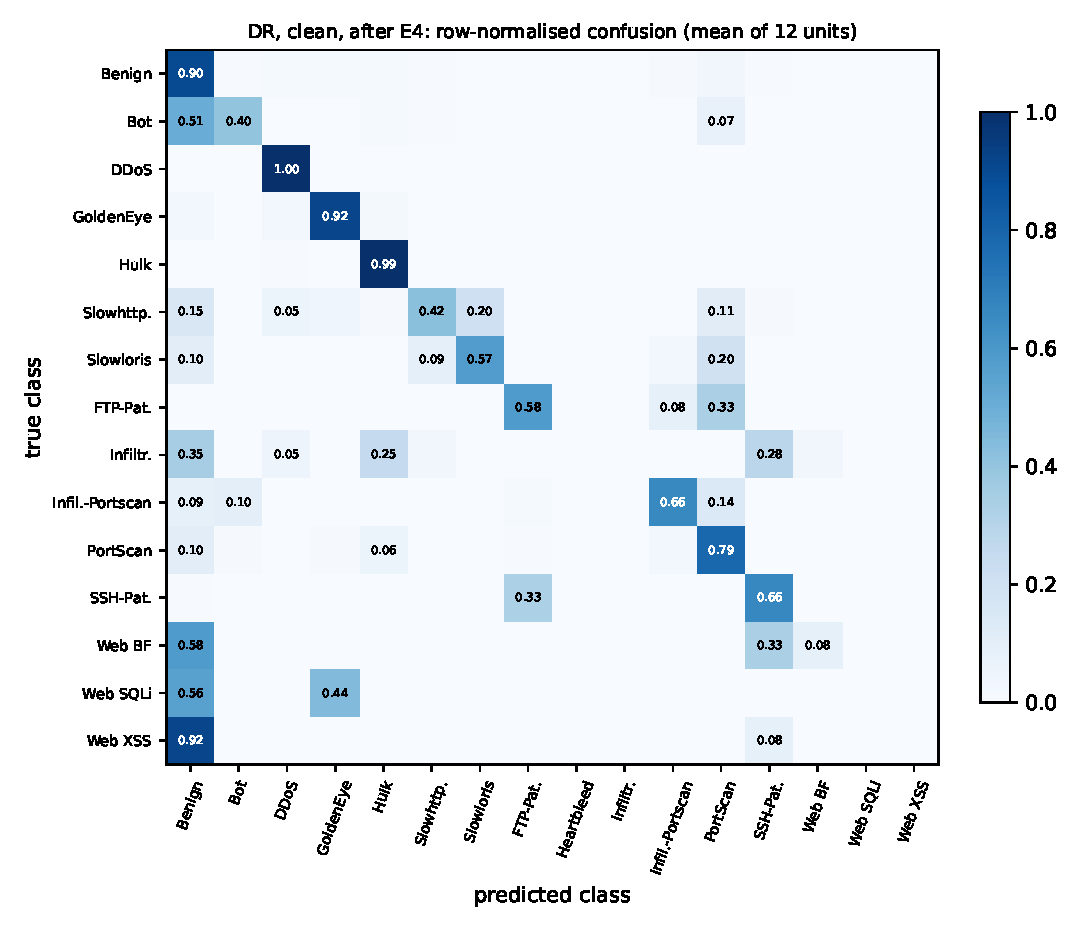
\includegraphics[width=0.75\linewidth]{figures/fig8-confusion-DR.pdf}
\caption{Row-normalised confusion matrix of the clean DR model after stage E4 (mean of 12 units); only classes present in the bank are shown as rows.}
\label{fig:conf}
\end{figure}
\begin{figure}[htbp]
\centering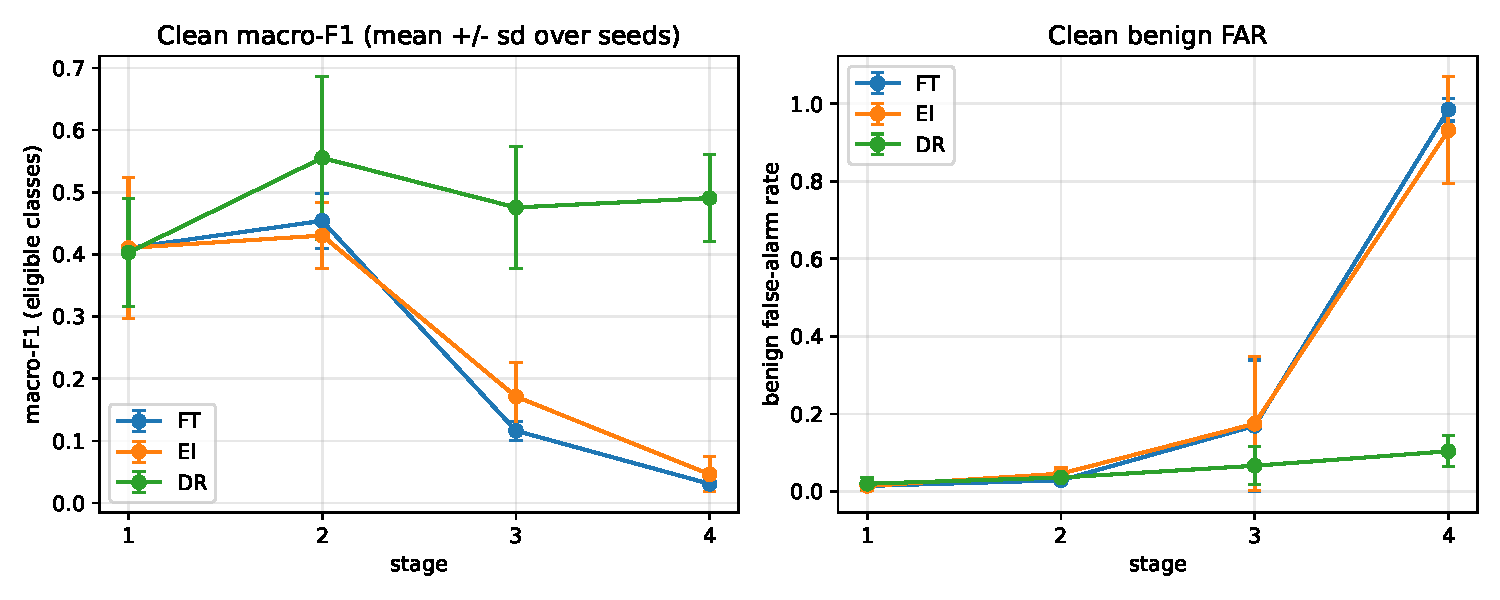
\includegraphics[width=\figw]{figures/fig1-clean-by-stage.pdf}
\caption{Clean macro-F1 (left) and benign false-alarm rate (right) after each stage, mean $\pm$ sd over 12 units.}
\label{fig:clean}
\end{figure}
\begin{figure}[htbp]
\centering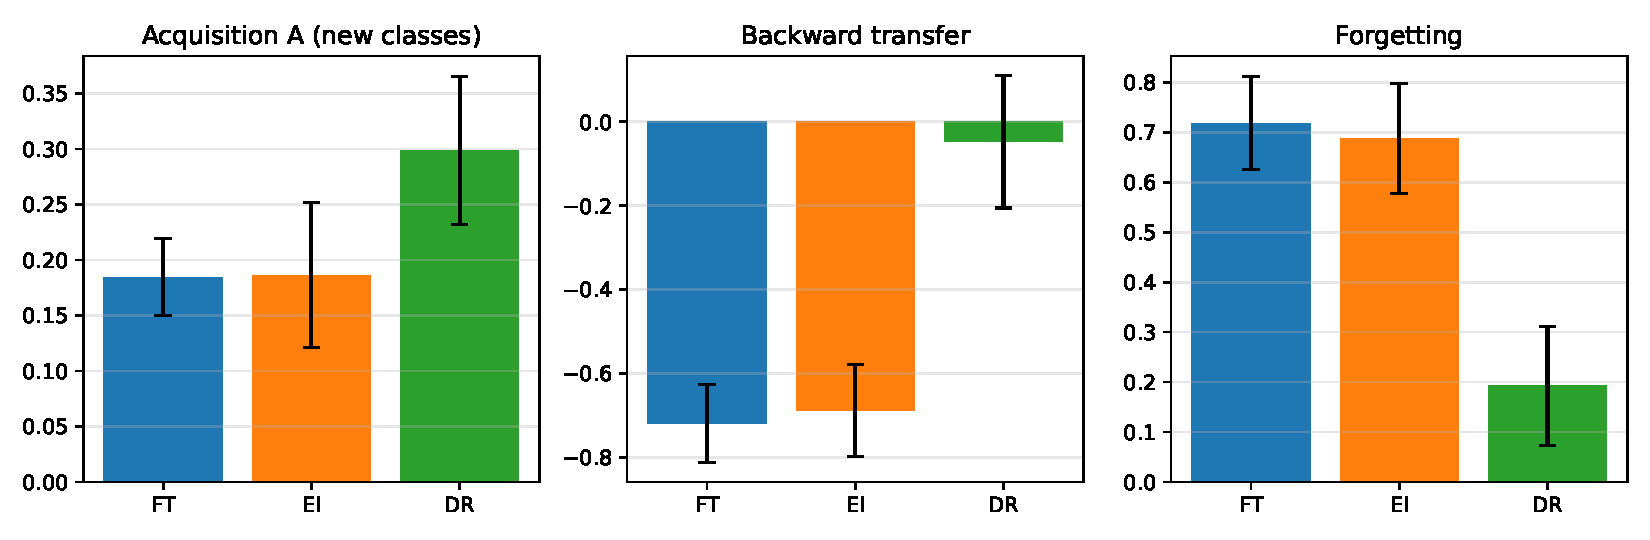
\includegraphics[width=\figw]{figures/fig2-retention-acquisition.pdf}
\caption{Acquisition of new classes, backward transfer and forgetting of the clean baselines (mean $\pm$ sd, 12 units).}
\label{fig:ret}
\end{figure}
Tables~\ref{tab:ess} and~\ref{tab:bin} give the essential detection metrics and Figure~\ref{fig:conf} the confusion matrix of DR. As a binary detector DR reaches a detection rate of 0.99 with a false-positive rate of 0.10 and precision 0.72 (the benign class is the largest in the bank, so precision depends on its prevalence), while FT and EI detect almost every attack only because they call almost every flow an attack (FPR 0.93--0.98). Without an attack, DR is the only learner that works across the four stages: final macro-F1 0.49, BWT close to zero and a benign false-alarm rate of 0.10. FT and EI collapse: after stage E4 they label 93--98\% of benign traffic as attack, forget about 0.7 of the earlier classes' recall and keep none of Hulk's recall. This is the expected behaviour of class-incremental learning without replay when the last stage is dominated by one large class; EI's penalty ($\lambda_E{=}100$) is too weak to prevent it, and Table~\ref{tab:abl} shows that stronger or weaker penalties do not change this. These two learners are therefore a lower bound, and their poisoning damage must be read against what they have left to lose.

The repository's own committed development runs, produced by a different implementation of the same protocol, give clean E4 macro-F1 of 0.018 (FT), 0.037 (EI) and 0.655 (DR) (three seeds). Our values for the same three partitions are 0.033, 0.053 and 0.434. The ordering agrees, FT and EI are at the floor in both, but our DR is clearly lower; we report this difference as measured and have not tuned toward the committed value. The 12-unit mean of 0.49 includes training replicates of the same partitions.

%=====================================================================
\section{Poisoning and Defences}\label{sec:def}
\subsection{RQ1: damage to the three learners}
\begin{table}[htbp]
\centering\footnotesize
\caption{Poisoning dose-response without a defence (mean over 12 units). Arm \texttt{kN-dX}: $N$ attacking clients each relabel a fraction $X$ of their Hulk rows; share = fraction of all stage-E2 Hulk rows flipped. $\Delta$rec = Hulk recall lost at E2; $H$ = Hulk recall lost at E4 relative to the same learner without attack; ASR = share of Hulk rows predicted benign at E4.}
\label{tab:dose}
\begin{tabularx}{\linewidth}{llrrrrrrrr}
\toprule
Learner & Arm & Share & Hulk rec.\ E2 & $\Delta$rec & Hulk rec.\ E4 & $H$ & ASR E4 & FAR E4 & Macro-F1\\
\midrule
FT & clean & 0.00 & 1.000 & 0.000 & 0.000 & 0.000 & 0.000 & 0.984 & 0.031\\
FT & k5-d0.25 & 0.25 & 1.000 & 0.000 & 0.000 & 0.000 & 0.000 & 1.000 & 0.028\\
FT & k1-d1 & 0.26 & 0.968 & 0.031 & 0.000 & 0.000 & 0.000 & 0.999 & 0.031\\
FT & k5-d0.5 & 0.50 & 0.506 & 0.494 & 0.000 & 0.000 & 0.000 & 1.000 & 0.028\\
FT & k3-d1 & 0.70 & 0.165 & 0.835 & 0.000 & 0.000 & 0.000 & 1.000 & 0.030\\
FT & k5-d0.9 & 0.90 & 0.000 & 1.000 & 0.000 & 0.000 & 0.000 & 1.000 & 0.023\\
EI & clean & 0.00 & 1.000 & 0.000 & 0.000 & 0.000 & 0.000 & 0.932 & 0.046\\
EI & k5-d0.25 & 0.25 & 0.999 & 0.000 & 0.000 & 0.000 & 0.000 & 1.000 & 0.038\\
EI & k1-d1 & 0.26 & 0.943 & 0.057 & 0.000 & 0.000 & 0.000 & 0.998 & 0.041\\
EI & k5-d0.5 & 0.50 & 0.470 & 0.530 & 0.000 & 0.000 & 0.000 & 0.994 & 0.036\\
EI & k3-d1 & 0.70 & 0.162 & 0.838 & 0.000 & 0.000 & 0.000 & 0.995 & 0.036\\
EI & k5-d0.9 & 0.90 & 0.000 & 1.000 & 0.000 & 0.000 & 0.000 & 0.997 & 0.032\\
DR & clean & 0.00 & 1.000 & 0.000 & 0.993 & 0.000 & 0.000 & 0.104 & 0.491\\
DR & k5-d0.25 & 0.25 & 1.000 & 0.000 & 0.962 & 0.032 & 0.030 & 0.101 & 0.474\\
DR & k1-d1 & 0.26 & 0.869 & 0.130 & 0.832 & 0.162 & 0.158 & 0.112 & 0.447\\
DR & k5-d0.5 & 0.50 & 0.387 & 0.612 & 0.209 & 0.785 & 0.783 & 0.087 & 0.427\\
DR & k3-d1 & 0.70 & 0.117 & 0.883 & 0.411 & 0.582 & 0.578 & 0.122 & 0.403\\
DR & k5-d0.9 & 0.90 & 0.000 & 1.000 & 0.000 & 0.993 & 0.992 & 0.091 & 0.393\\
\bottomrule
\end{tabularx}
\end{table}
\begin{figure}[htbp]
\centering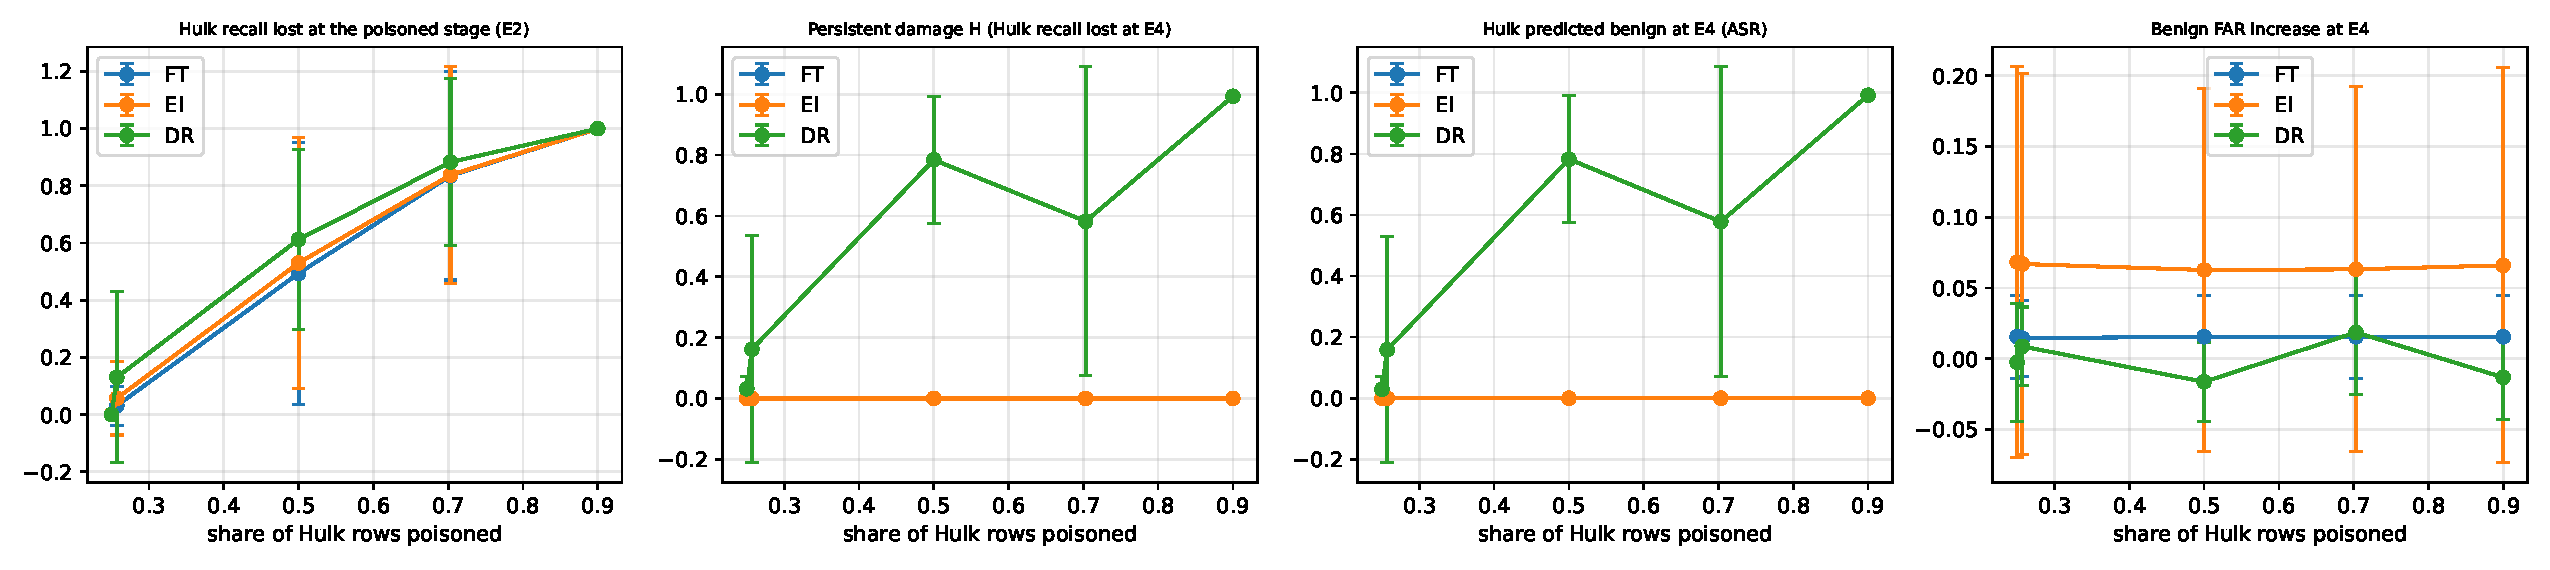
\includegraphics[width=\figw]{figures/fig3-dose-response.pdf}
\caption{Dose-response without a defence. The horizontal axis is the measured share of Hulk rows poisoned; panels show immediate Hulk recall loss, persistent damage $H$, attack success rate at E4 and the increase in benign FAR (mean $\pm$ sd, 12 units).}
\label{fig:dose}
\end{figure}
Poisoning works once enough clients take part (Table~\ref{tab:dose}, Figure~\ref{fig:dose}). One attacker holding about a quarter of the Hulk rows has little effect (DR loses 0.13 of Hulk recall at E2), while five attackers relabelling half of the Hulk rows cost every learner about half of its Hulk recall at the poisoned stage (0.49 for FT, 0.53 for EI, 0.61 for DR) and almost all of it at 90\% (1.00). Federated averaging dilutes a minority attacker: this is the same finding as in the label-flipping study P5 \cite{lavaur}, which reported small relative success for a single attacker among ten clients.

The learners differ after the attacker is withdrawn. FT and EI have already lost Hulk at E4 in the clean runs, so their $H$ is zero by construction and their damage appears only in the immediate loss. DR keeps Hulk without an attack (recall 0.99), but loses persistently: $H=0.79$ at 50\% poisoning and $0.99$ at 90\%. The poisoned records stay in the replay memories (630 on average at 50\%), which is why the error survives the stages in which no poison and no fresh Hulk data arrive. One result is not monotone: at about 70\% poisoning (three attackers) $H=0.58$, lower than at 50\%, with a wide spread over units. We did not isolate the reason and report it as an unexplained observation.

Family C1 confirms the learner differences only where they are measurable: six of the 30 tests are significant after Holm correction, all comparing DR with FT or EI on persistent damage in the three arms with five attackers (Table~\ref{tab:c1}). The tests on immediate damage show no significant difference between learners, consistent with all three being fooled when the attack is strong.

\begin{table}[htbp]
\centering\footnotesize
\caption{Confirmatory family C1: the six learner-pair comparisons that remain significant after Holm correction (30 tests in the family). All are DR compared with FT or EI on persistent damage $H$.}
\label{tab:c1}
\begin{tabularx}{\linewidth}{llllYrr}
\toprule
Comparison & Endpoint & Arm & Mean diff. & 95\% CI & $r$ & Holm $p$\\
\midrule
DR minus EI & H & k5-d0.25 & +0.032 & [+0.012, +0.056] & +0.97 & 0.025\\
DR minus EI & H & k5-d0.5 & +0.785 & [+0.668, +0.891] & +1.00 & 0.015\\
DR minus EI & H & k5-d0.9 & +0.993 & [+0.990, +0.997] & +1.00 & 0.015\\
DR minus FT & H & k5-d0.25 & +0.032 & [+0.012, +0.057] & +0.97 & 0.025\\
DR minus FT & H & k5-d0.5 & +0.785 & [+0.666, +0.893] & +1.00 & 0.015\\
DR minus FT & H & k5-d0.9 & +0.993 & [+0.990, +0.997] & +1.00 & 0.015\\
\bottomrule
\end{tabularx}
\end{table}

\subsection{RQ2: class-aware versus global admission}
Figure~\ref{fig:def} shows the four rules across the attack arms, and Figure~\ref{fig:adm} the share of poison each admitted.
\begin{figure}[htbp]
\centering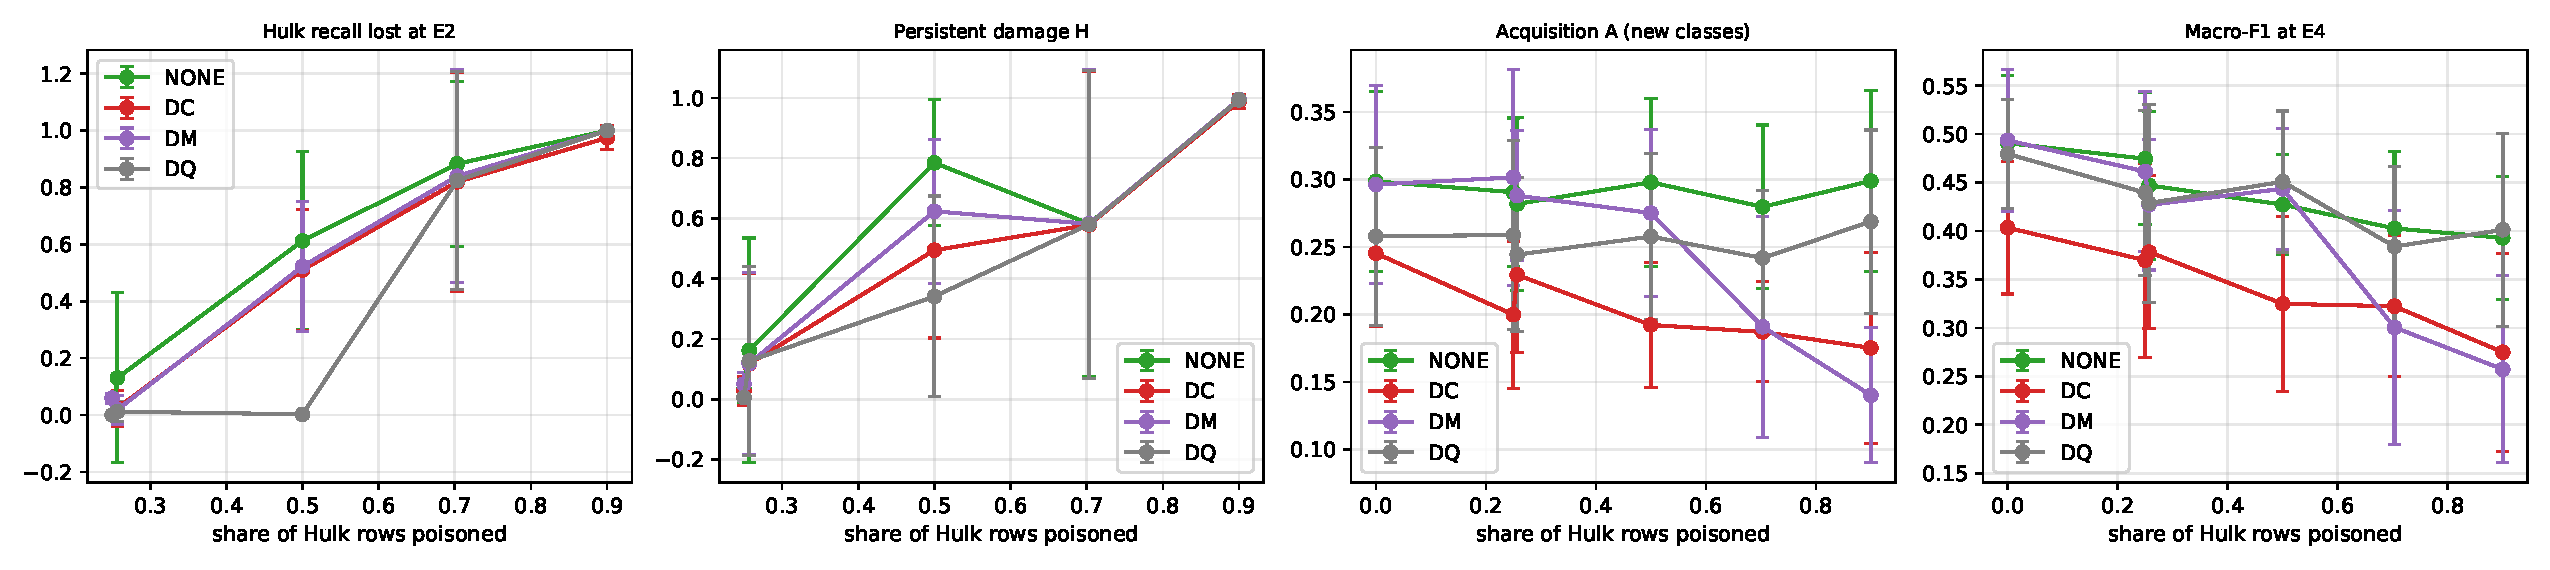
\includegraphics[width=\figw]{figures/fig4-defences.pdf}
\caption{Admission rules on the DR learner by poisoned share: immediate recall loss, persistent damage $H$, acquisition $A$ and macro-F1 at E4 (mean $\pm$ sd, 12 units).}
\label{fig:def}
\end{figure}
\begin{table}[htbp]
\centering\footnotesize
\caption{Admission rules on the strongest arm (five attackers, dose 0.9; 12 units). Every rule admits the same number of rows per client.}
\label{tab:adm}
\begin{tabularx}{\linewidth}{lYYYYYYYY}
\toprule
Rule & Rows admitted & New-class rows kept & Poisoned rows admitted & Poison left in memory & $\Delta$rec & $H$ & $A$ & Macro-F1\\
\midrule
NONE & 100.0\% & 100.0\% & 100.0\% & 1115 & 1.000 & 0.993 & 0.299 & 0.393\\
DC & 79.0\% & 100.0\% & 77.5\% & 1037 & 0.974 & 0.988 & 0.175 & 0.275\\
DM & 79.0\% & 9.5\% & 94.0\% & 1265 & 1.000 & 0.995 & 0.140 & 0.257\\
DQ & 79.0\% & 100.0\% & 75.0\% & 992 & 1.000 & 0.994 & 0.269 & 0.401\\
\bottomrule
\end{tabularx}
\end{table}
\begin{figure}[htbp]
\centering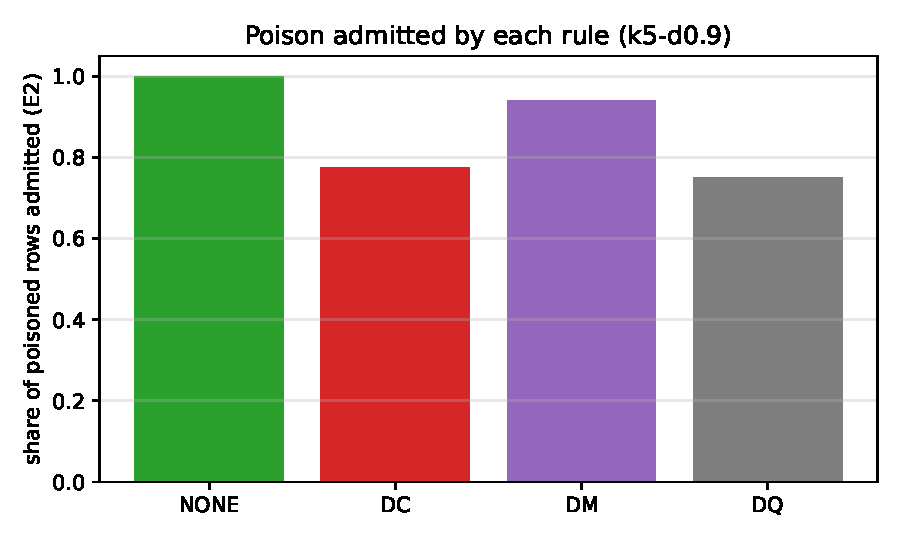
\includegraphics[width=0.55\linewidth]{figures/fig5-poison-admitted.pdf}
\caption{Share of the poisoned rows each rule admitted in stage E2 (five attackers, dose 0.9).}
\label{fig:adm}
\end{figure}
Under the strongest attack, DC and DQ admit 77.5\% and 75.0\% of the poisoned rows and DM admits 94\%, against 100\% with no admission. This is a small reduction, and it does not lower persistent damage: $H$ is 0.99 for every rule (Table~\ref{tab:adm}), because enough poisoned rows still enter the memory and training. The class-aware quota does protect legitimate evidence: DC and DQ keep every row of newly arriving classes, while the global ranking DM keeps only 9.5\% of them, since new classes have a high loss under a model that has not yet learned them. In terms of acquisition DC is slightly better than DM at this arm ($+0.035$), but that difference is not significant.

\begin{table}[htbp]
\centering\footnotesize
\caption{Confirmatory family C2: DC minus DM, paired over 12 units (Wilcoxon signed-rank, Holm-adjusted within the family; CI = 95\% bootstrap over units; $r$ = rank-biserial correlation). Endpoints $\Delta$rec and $H$ are damage measures (lower is better); $A$ is acquisition (higher is better).}
\label{tab:c2}
\begin{tabularx}{\linewidth}{llrYrrr}
\toprule
Endpoint & Arm & Mean diff. & 95\% CI & $r$ & Holm $p$ & Sig.\\
\midrule
A (acquisition) & clean & -0.051 & [-0.069, -0.035] & -1.00 & 0.008 & yes\\
A (acquisition) & k5-d0.25 & -0.102 & [-0.131, -0.076] & -1.00 & 0.008 & yes\\
A (acquisition) & k1-d1 & -0.059 & [-0.083, -0.034] & -0.92 & 0.029 & yes\\
A (acquisition) & k5-d0.5 & -0.083 & [-0.110, -0.059] & -1.00 & 0.008 & yes\\
A (acquisition) & k3-d1 & -0.004 & [-0.035, +0.025] & +0.00 & 1.000 & no\\
A (acquisition) & k5-d0.9 & +0.035 & [+0.015, +0.053] & +0.85 & 0.075 & no\\
H & k5-d0.25 & -0.023 & [-0.051, +0.006] & -0.46 & 1.000 & no\\
H & k1-d1 & -0.001 & [-0.004, +0.001] & -0.41 & 1.000 & no\\
H & k5-d0.5 & -0.129 & [-0.255, -0.015] & -0.54 & 0.989 & no\\
H & k3-d1 & -0.004 & [-0.012, +0.001] & -0.18 & 1.000 & no\\
H & k5-d0.9 & -0.007 & [-0.023, +0.003] & +0.10 & 1.000 & no\\
dRec & k5-d0.25 & -0.059 & [-0.069, -0.050] & -1.00 & 0.008 & yes\\
dRec & k1-d1 & +0.006 & [-0.000, +0.014] & +0.33 & 1.000 & no\\
dRec & k5-d0.5 & -0.013 & [-0.151, +0.123] & -0.03 & 1.000 & no\\
dRec & k3-d1 & -0.020 & [-0.052, -0.000] & -0.58 & 1.000 & no\\
dRec & k5-d0.9 & -0.025 & [-0.050, -0.006] & -0.64 & 0.801 & no\\
clean FAR (E4) & clean & +0.072 & [+0.051, +0.094] & +1.00 & 0.008 & yes\\
\bottomrule
\end{tabularx}
\end{table}
Table~\ref{tab:c2} shows that the confirmatory result is, however, not the one Phase 2 expected. At the clean arm and at the weak and medium attacks DC acquires \emph{less} than DM by 0.05--0.10 in $A$, and DC raises clean false alarms by 0.07. The random control DQ with the same quota reaches macro-F1 0.40 and $A=0.27$ at the strongest arm, against 0.28 and 0.18 for DC. The comparison suggests that the class-aware quota is the useful ingredient, while ranking the rows by loss inside the quota removes hard but legitimate rows; this is an interpretation of the pattern, not a tested mechanism. No test on persistent damage is significant, so we cannot claim that class-aware admission is safer than the matched global filter.

\subsection{RQ3: cost}
\begin{table}[htbp]
\centering\footnotesize
\caption{Cost per complete run (four stages, 12 rounds each, five clients; Tesla T4, four runs in parallel).}
\label{tab:cost}
\begin{tabularx}{\linewidth}{lYYYY}
\toprule
Learner & Wall time (s) & Model (KB) & Communication (MB) & Replay memory (KB)\\
\midrule
DR & 53 & 75.6 & 35.5 & 940\\
EI & 38 & 75.6 & 35.5 & 0\\
FT & 20 & 75.6 & 35.5 & 0\\
\bottomrule
\end{tabularx}
\end{table}
\begin{figure}[htbp]
\centering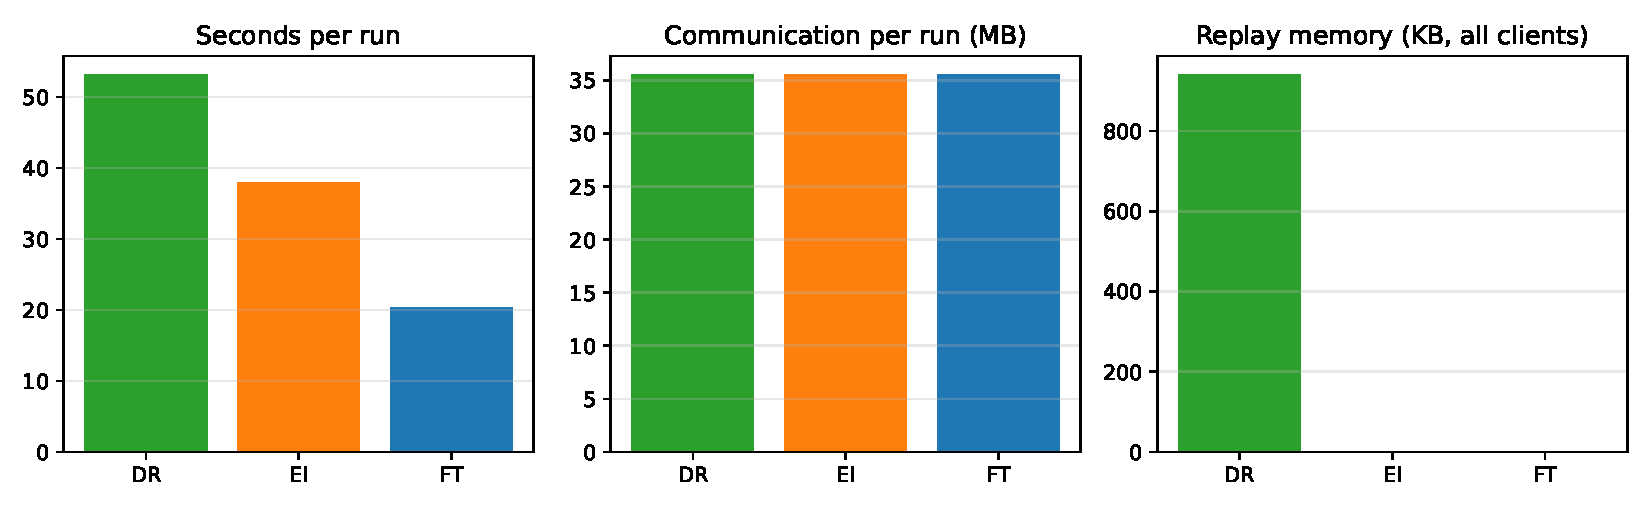
\includegraphics[width=\figw]{figures/fig7-cost.pdf}
\caption{Wall time, communicated bytes and replay memory per run.}
\label{fig:cost}
\end{figure}
Table~\ref{tab:cost} and Figure~\ref{fig:cost} give the cost. Replay costs about 2.6 times the time of fine-tuning and 1.4 times that of EI in our implementation, plus 940~KB of memory across the five clients. Communication is identical for all learners (35.5~MB per run), because the same model is exchanged in every round.

%=====================================================================
\section{Ablation Studies}\label{sec:abl}
\begin{table}[htbp]
\centering\footnotesize
\caption{Ablations at the poisoned arm five attackers $\times$ 0.5 (12 units each; every variant has its own clean twin, so damage is measured against its own clean run). Poison left = poisoned records still in the replay memories at the end.}
\label{tab:abl}
\begin{tabularx}{\linewidth}{lYYYYYYY}
\toprule
Setting & $\Delta$rec & $H$ & Macro-F1 & Clean F1 & FAR E4 & $A$ & Poison left\\
\midrule
DR reference & 0.612 & 0.785 & 0.427 & 0.491 & 0.087 & 0.298 & 630\\
DR: no logit-matching (lam\_z=0) & 0.430 & 0.637 & 0.401 & 0.453 & 0.156 & 0.270 & 630\\
DR: no replay-label term (lam\_y=0) & 0.883 & 0.000 & 0.055 & 0.083 & 0.789 & 0.189 & 630\\
DR: FIFO memory & 0.561 & 0.000 & 0.056 & 0.121 & 0.791 & 0.204 & 0\\
DR: memory 100/client & 0.355 & 0.513 & 0.344 & 0.386 & 0.171 & 0.263 & 116\\
DR: memory 1000/client & 0.698 & 0.741 & 0.471 & 0.522 & 0.085 & 0.301 & 1248\\
DR+DC reference & 0.510 & 0.495 & 0.325 & 0.403 & 0.418 & 0.192 & 542\\
DR+DC: quota q=0.5 & 0.306 & 0.450 & 0.292 & 0.396 & 0.490 & 0.168 & 419\\
DR+DC: quota q=0.9 & 0.716 & 0.641 & 0.336 & 0.457 & 0.312 & 0.205 & 611\\
DR+DC: small-class threshold 5 & 0.510 & 0.495 & 0.325 & 0.403 & 0.418 & 0.192 & 542\\
DR+DC: small-class threshold 100 & 0.510 & 0.495 & 0.325 & 0.406 & 0.418 & 0.192 & 542\\
EI reference (lam\_E=100) & 0.530 & 0.000 & 0.036 & 0.046 & 0.994 & 0.185 & 0\\
EI: lam\_E=10 & 0.500 & 0.000 & 0.033 & 0.074 & 1.000 & 0.198 & 0\\
EI: lam\_E=1000 & 0.489 & 0.000 & 0.036 & 0.040 & 1.000 & 0.160 & 0\\
\bottomrule
\end{tabularx}
\end{table}
\begin{figure}[htbp]
\centering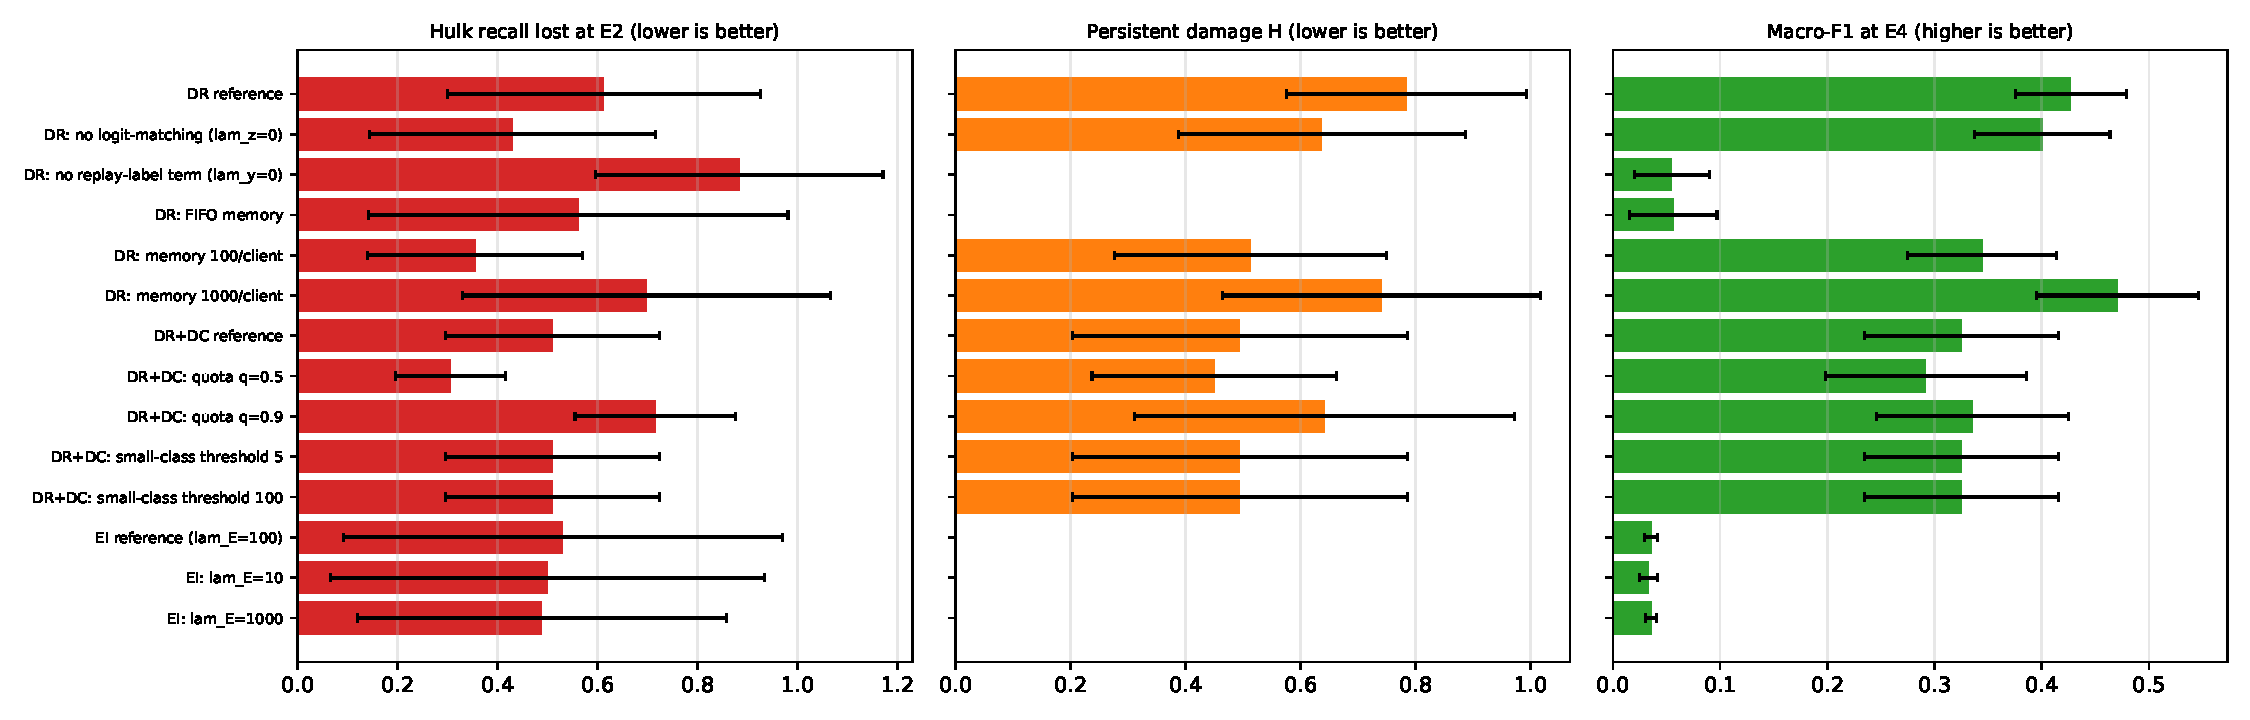
\includegraphics[width=\figw]{figures/fig6-ablations.pdf}
\caption{Ablations at five attackers $\times$ 0.5: immediate Hulk recall loss, persistent damage $H$ and macro-F1 at E4 (mean $\pm$ sd, 12 units).}
\label{fig:abl}
\end{figure}
\begin{itemize}
\item \textbf{Replay-label term.} Removing it ($\lambda_y=0$) collapses DR to macro-F1 0.055 and a false-alarm rate of 0.79: replay then keeps only the logit-matching signal, which is not enough to retain classes. Its $H$ of zero reflects the clean twin having already lost Hulk, not robustness.
\item \textbf{Memory eviction.} FIFO memory also collapses retention (macro-F1 0.056), but it leaves no poisoned records, since the old records are overwritten. Reservoir memory keeps retention and keeps the poison (630 records). Retention and poison persistence therefore come from the same mechanism.
\item \textbf{Memory size.} A memory of 100 records per client lowers persistent damage ($H=0.51$) and macro-F1 (0.34); 1,000 records raise macro-F1 to 0.47 and keep more poison (1,248 records, $H=0.74$).
\item \textbf{Logit matching.} Removing it lowers $H$ slightly (0.64) and macro-F1 slightly (0.40 against 0.43).
\item \textbf{Admission settings.} A smaller quota ($q=0.5$) gives the lowest $H$ among the DC settings (0.45) at the cost of macro-F1; the small-class threshold $n_{\min}$ has no effect at all (identical to the reference).
\item \textbf{EI strength.} $\lambda_E$ between 10 and 1,000 does not change the collapse of EI.
\end{itemize}

%=====================================================================
\section{Comparison with Existing Research}\label{sec:lit}
The reviewed studies use different datasets, class sets, client counts, metrics and attack models, so their reported numbers cannot be compared with ours and we make no claim of higher accuracy. Table~\ref{tab:lit} places our observations next to what each study reports, using the figures stated in the Phase 2 review, and Table~\ref{tab:fair} lists the nearest comparable numbers with the reasons a fair comparison is not possible. Where a dataset or metric is shared, our headline numbers are \emph{lower}, not higher, than the published ones; our setting is harder (16 classes arriving over four stages, five federated clients, poisoned labels) and the published numbers are for easier or different tasks.

\begin{table}[htbp]
\centering\footnotesize
\caption{Qualitative comparison with the reviewed studies (their reported figures are theirs and are not comparable with ours).}
\label{tab:lit}
\begin{tabularx}{\linewidth}{L{2.4cm}L{4.3cm}Y}
\toprule
Study & Reports & Relation to our results\\
\midrule
P5, Lavaur et al.\ \cite{lavaur} & Label flipping in federated IDS; one attacker of ten gives relative success below 0.1; damage grows with participation; fixed binary model & Same dilution of a single attacker (our one-attacker arms) and growing damage with participation (our 3 and 5 attacker arms); we add class-incremental learning and replay persistence\\
P9, Guo et al.\ \cite{guo} & Memory selection in continual IDS; removing the memory component drops F1 from 82.1 to 76.4\%; notes replay could be exploited & Our ablations show replay is both necessary for retention and the carrier of poisoned knowledge; we test the exploitation they name\\
P8, Cerasuolo et al.\ \cite{cerasuolo} & Benchmark of FT, replay, LwF, EWC and others, clean and centralised & Our clean ordering (replay $\gg$ EWC-style $\approx$ FT) is consistent with replay-based methods being the strong baseline; we add poisoning and federation\\
P13, Nguyen and Park \cite{elgnn} & EWC-based continual IDS on two binary tasks, clean data & Our EWC-style learner does not prevent forgetting in a 16-class four-stage setting\\
P11, Banbhrani et al.\ \cite{flzt} & Trust filter rejects 4.6\% of honest clients; binary, static classes & Our admission rules also remove honest evidence: DM discards 90\% of new-class rows under attack and DC lowers acquisition\\
P10, Latif and Djenouri \cite{amm} & Rare class sometimes absorbed into normal traffic; static classes & Consistent: rows of new, rare classes are the ones a loss-ranked filter removes\\
P7, Sameera et al.\ \cite{wei} & Needs at least 90\% trusted auxiliary data; static classes & Our admission rules use no trusted data, and none removes persistent damage\\
P12, Abhijit et al.\ \cite{rare} & New-class trigger from client-reported performance, all clients trusted & We poison during class acquisition and show the damage persists; the trigger is a plausible attack surface (not tested)\\
P4, Carillo et al.\ \cite{carillo} & Federated class-incremental IDS with honest clients; new classes learned poorly & Our clean acquisition scores ($A\approx0.19$--$0.30$) show the same difficulty with new classes\\
\bottomrule
\end{tabularx}
\end{table}


\begin{table}[htbp]
\centering\footnotesize
\caption{Nearest comparable published results and why they are not directly comparable. Their numbers are as stated in the Phase 2 review.}
\label{tab:fair}
\begin{tabularx}{\linewidth}{L{1.5cm}L{2.2cm}L{3.3cm}L{3.0cm}Y}
\toprule
Study & Shared with ours & Their result & Our nearest value & Limit on a fair comparison\\
\midrule
P9 \cite{guo} & CICIDS2017, continual stages & Accuracy 83.4\%, F1 82.1\% (five stages) & Accuracy 0.911, macro-F1 0.491 (DR, four stages) & Different stage definition and class set; our accuracy is dominated by the benign class; theirs is not federated and uses a different split\\
P11 \cite{flzt} & CICIDS2017, FL, poisoning & Accuracy 97.8\%; 89.3\% under 30\% sign-flipping; 4.6\% honest clients rejected & Binary accuracy 0.916, detection rate 0.993, FPR 0.104 (clean DR) & Their model is binary with static classes and no continual learning; ours is class-incremental\\
P13 \cite{elgnn} & CICIDS2017, EWC & About 85\% after two tasks (CICIDS2017 to UNSW-NB15) & EI macro-F1 0.046 (collapses) & Two binary tasks on two datasets, graph model; ours has 16 classes in four stages\\
P6 \cite{cnd} & CICIDS2017, continual & 1.93$\times$ over LwF in novelty-score F1 & Not applicable & Unlabelled novelty detection with a benign-only start; ours is supervised\\
P5 \cite{lavaur} & Label flipping in FL & Relative attack success below 0.1 with one attacker of ten & DR attack success 0.16 at one attacker (about 26\% of Hulk rows), 0.78 at 50\% & Different datasets (NF-v2 data), binary model, ten clients; ours five clients, per-family success\\
P7 \cite{wei} & Poisoning defence & Clean F1 89.79\% and 94.18\% & Not applicable & Other datasets; requires trusted auxiliary data that our rules do not use\\
\bottomrule
\end{tabularx}
\end{table}

%=====================================================================
\section{Analysis and Discussion}\label{sec:disc}
\textbf{RQ1.} Replay is the only learner that retains earlier families, and it is also the only one whose damage persists measurably, because the poisoned records stay in memory. The strength of the attack, not the number of attackers alone, decides the harm: a minority attacker is diluted by federated averaging, whereas five attackers relabelling half of the Hulk rows already cost every learner about half of its Hulk recall at the poisoned stage. For DR the loss survives the withdrawal of the attacker (0.79 at 50\%, 0.99 at 90\%).

\textbf{RQ2.} None of the tested admission rules reduced persistent damage, and the confirmatory tests of DC against DM show lower, not higher, acquisition for DC at the clean and weaker arms. The class-aware quota does what it was designed for (all new-class rows kept, against 9.5\% for the global ranking at the strongest attack), but the loss-based choice inside the quota costs accuracy; the random quota DQ was as good or better than DC on macro-F1 and acquisition. A class-aware rule based on loss is therefore not a safe default for this attack.

\textbf{RQ3.} Retention and poison persistence share one mechanism: the replay memory. The replay-label term is essential, FIFO eviction removes the poison but also the retention, and memory size trades the two. Replay costs about 2.6 times the time of fine-tuning, and communication is unchanged.


\subsection{Do the results address the research gap and objectives?}
\textbf{Gap G1 (poisoning during class acquisition, and its persistence).} Yes, partly. We measured the immediate and the persistent damage of a poisoned acquisition stage for three learners over six attack arms and found that replay keeps the poison after the attacker withdraws (RQ1 answered with 12 paired units). The finding is limited to one dataset and one attack pattern.

\textbf{Gap G2 (defences that reject legitimate new evidence).} Yes, and the answer is negative for the proposed rule. The global matched filter does discard legitimate evidence (9.5\% of new-class rows kept under the strongest attack), the class-aware quota keeps it, but the class-aware rule did not reduce persistent damage and cost acquisition at the clean and weaker arms. The objective of a defence that protects without blocking new families was therefore \emph{not} met by DC in our setting.

\textbf{Gap G3 (mechanism and cost).} Yes. Retention and poison persistence share the replay memory; the replay-label term and the eviction rule are decisive; cost is wall time, memory bytes and unchanged communication.

\subsection{Strengths and limitations of the proposed class-aware rule}
\textbf{Strengths.} It admits exactly the same volume as the matched global filter, needs no trusted data, keeps every row of a newly arriving class, and removes slightly more poison (77.5\% of the poisoned rows admitted against 94\% for DM at the strongest arm). The comparison with the random quota DQ isolates its design choices.
\textbf{Limitations.} Its loss ranking inside the quota lowers acquisition and macro-F1 relative to both no admission and DQ, raises clean false alarms by 0.07, and does not lower persistent damage. It protects only against poison that is visible to the current model's loss; poison already stored in the replay memory is not removed by admission at later stages.

\subsection{Limitations}
\begin{itemize}
\item \textbf{Single dataset, single attack pattern} (Hulk relabelled benign in stage E2, withdrawn afterwards); development bank only; the sealed final evaluation was not run.
\item \textbf{Units are not independent.} The 12 units are three ownership partitions with four training replicates each; replicates within a partition share their client ownership, so the tests overstate independence. They measure training variability on a fixed development bank, not variability between captures.
\item \textbf{Weak baselines.} FT and EI collapse even without an attack, so their poisoning damage is bounded by what is left to lose. Interpret C1 together with Table~\ref{tab:baselines}.
\item \textbf{DR level.} Our clean DR is below the committed repository value (0.434 against 0.655 on the same partitions); the difference between the two implementations was not resolved.
\item \textbf{Unexplained pattern.} Persistent damage at about 70\% poisoning is lower than at 50\%.
\item \textbf{Explanations.} Statements about why DC loses acquisition (loss ranking removes hard legitimate rows) are interpretations supported by the DQ control, not tested mechanisms. CPU and GPU runs are not bit-identical; all reported runs used the GPU.
\item \textbf{Not run.} The external dataset check, the unmatched global filter DG, inference latency and the poisoned-memory clone diagnostic from Phase 2.
\end{itemize}

\subsection{Conclusion}
In a federated continual intrusion detector, replay is required to retain earlier attack families, but it also keeps poisoned labels in memory after the attacker has stopped. A minority attacker is diluted by averaging, and the admission rules we tested, including a class-aware quota, did not remove the persistent damage; the quota protects new classes better than a global filter, but ranking by loss within it costs accuracy. A defence that clears poison from the replay memory without erasing retention is therefore the open problem our results point to.

%=====================================================================
\section*{Availability and Requirement Map}
All material is in the folder \texttt{phase3-implementation/} of the project repository. Code: \texttt{src/p3lib.py} and \texttt{src/p3parallel.py}; the notebook that was run on Kaggle: \texttt{notebooks/phase3-experiments.ipynb}; results of the final run in \texttt{results/final-run/}: \texttt{part-a-dataset.zip} (dataset and preprocessing report), \texttt{part-b-experiment-runs.zip} (the 696 run files) and \texttt{part-c-analysis.zip} (tables, figures and statistics), also unpacked in \texttt{analysis/} and \texttt{dataset-report/}. A plain-language project description is in \texttt{docs/project-brief.md}. Each figure is saved with its source table, and every run file is hashed in \texttt{run-file-hashes.json}.

\begin{table}[htbp]
\centering\footnotesize
\caption{Phase 3 requirements and where they are satisfied.}
\begin{tabularx}{\linewidth}{L{0.6cm}L{4.4cm}Y}
\toprule
\# & Requirement & Where\\
\midrule
1 & Implementation of the methodology & Section~\ref{sec:impl}; \texttt{src/p3lib.py}, \texttt{src/p3parallel.py}\\
2 & Dataset and preprocessing & Section~\ref{sec:data}, Table~\ref{tab:classes}\\
3 & Baseline evaluation & Section~\ref{sec:base}, Tables~\ref{tab:baselines}--\ref{tab:bin}, Figures~\ref{fig:clean}--\ref{fig:ret}, \ref{fig:conf}\\
4 & Graphical results & Figures~\ref{fig:clean}--\ref{fig:cost}\\
5 & Comparison with existing research & Section~\ref{sec:lit}, Tables~\ref{tab:lit}--\ref{tab:fair}\\
6 & Ablation studies & Section~\ref{sec:abl}, Table~\ref{tab:abl}, Figure~\ref{fig:abl}\\
7 & Results analysis and discussion & Sections~\ref{sec:def} and~\ref{sec:disc} (including the gap and objective check), Tables~\ref{tab:dose}--\ref{tab:c2}\\
\bottomrule
\end{tabularx}
\end{table}

\begin{thebibliography}{99}
\bibitem{phase1} Saneedullah and A. Bilal, \enquote{Continual learning for network security: Phase 1 literature review and research gap identification,} Computer Networks course report, FAST-NUCES, 2026.
\bibitem{ge} J. Ge, Y. Feng, and K. Sakurai, \enquote{A stage-wise framework using class-incremental learning for unknown DoS attack detection,} \emph{Future Internet}, vol. 18, no. 3, Art. 145, 2026. \url{https://doi.org/10.3390/fi18030145}.
\bibitem{wu} Z. Wu, B. He, Z. Si, C. Qiu, X. Liao, and C. Su, \enquote{Communication-efficient federated class-incremental intrusion detection for edge IoT networks,} \emph{Sensors}, vol. 26, no. 14, Art. 4630, 2026. \url{https://doi.org/10.3390/s26144630}.
\bibitem{luo} F. Luo, S. Fan, X. Li, and W. Xu, \enquote{Adaptive feature distillation-based continuous authentication against RF fingerprint drift for power equipment,} \emph{Future Internet}, vol. 18, no. 9, Art. 457, 2026. \url{https://doi.org/10.3390/fi18090457}.
\bibitem{carillo} R. Carillo, F. Cerasuolo, G. Bovenzi, D. Ciuonzo, and A. Pescap\`e, \enquote{A federated and incremental network intrusion detection system for IoT emerging threats,} \emph{IEEE Trans. Network and Service Management}, vol. 23, pp. 3865--3880, 2026. \url{https://doi.org/10.1109/TNSM.2026.3675031}.
\bibitem{lavaur} L. Lavaur, Y. Busnel, and F. Autrel, \enquote{Investigating the impact of label-flipping attacks against federated learning for collaborative intrusion detection,} \emph{Computers \& Security}, vol. 156, Art. 104462, 2025. \url{https://doi.org/10.1016/j.cose.2025.104462}.
\bibitem{cnd} S. Fuhrman, O. Gungor, and T. Rosing, \enquote{CND-IDS: Continual novelty detection for intrusion detection systems,} in \emph{Proc. 62nd ACM/IEEE Design Automation Conference (DAC)}, 2025, pp. 1--7. \url{https://doi.org/10.1109/DAC63849.2025.11132541}.
\bibitem{wei} Sameera K. M., Vinod P., A. Rocha, Rafidha Rehiman K. A., and M. Conti, \enquote{WeiDetect: Weibull distribution-based defense against poisoning attacks in federated learning for network intrusion detection systems,} \emph{J. Information Security and Applications}, vol. 95, Art. 104275, 2025. \url{https://doi.org/10.1016/j.jisa.2025.104275}.
\bibitem{cerasuolo} F. Cerasuolo, G. Bovenzi, D. Ciuonzo, and A. Pescap\`e, \enquote{Attack-adaptive network intrusion detection systems for IoT networks through class incremental learning,} \emph{Computer Networks}, vol. 263, Art. 111228, 2025. \url{https://doi.org/10.1016/j.comnet.2025.111228}.
\bibitem{guo} C. Guo, X. Li, J. Cheng, S. Yang, and H. Gong, \enquote{Continual learning for intrusion detection under evolving network threats,} \emph{Future Internet}, vol. 17, no. 10, Art. 456, 2025. \url{https://doi.org/10.3390/fi17100456}.
\bibitem{amm} S. Latif and D. Djenouri, \enquote{Adaptive multi-model hierarchical federated learning for robust IoT intrusion detection,} \emph{Sensors}, vol. 26, no. 10, Art. 3198, 2026. \url{https://doi.org/10.3390/s26103198}.
\bibitem{flzt} S. K. Banbhrani, C. Wei, and M. Asad, \enquote{Trust-aware federated learning for privacy-preserving IoT intrusion detection,} \emph{Electronics}, vol. 15, no. 20, Art. 4584, 2026. \url{https://doi.org/10.3390/electronics15204584}.
\bibitem{rare} C. S. Abhijit, Y. A. Jerusha, S. P. Syed Ibrahim, and V. Varadharajan, \enquote{Federated transfer learning for rare attack class detection in network intrusion detection systems,} \emph{Scientific Reports}, vol. 15, Art. 33797, 2025. \url{https://doi.org/10.1038/s41598-025-02068-x}.
\bibitem{elgnn} T.-T. Nguyen and M. Park, \enquote{EL-GNN: A continual-learning-based graph neural network for task-incremental intrusion detection systems,} \emph{Electronics}, vol. 14, no. 14, Art. 2756, 2025. \url{https://doi.org/10.3390/electronics14142756}.
\bibitem{fedavg} B. McMahan, E. Moore, D. Ramage, S. Hampson, and B. Ag\"uera y Arcas, \enquote{Communication-efficient learning of deep networks from decentralized data,} in \emph{Proc. AISTATS}, PMLR, vol. 54, pp. 1273--1282, 2017.
\bibitem{ewc} J. Kirkpatrick et al., \enquote{Overcoming catastrophic forgetting in neural networks,} \emph{Proc. National Academy of Sciences}, vol. 114, no. 13, pp. 3521--3526, 2017. \url{https://doi.org/10.1073/pnas.1611835114}.
\bibitem{der} P. Buzzega, M. Boschini, A. Porrello, D. Abati, and S. Calderara, \enquote{Dark experience for general continual learning: A strong, simple baseline,} in \emph{Advances in Neural Information Processing Systems}, vol. 33, pp. 15920--15930, 2020.
\bibitem{vitter} J. S. Vitter, \enquote{Random sampling with a reservoir,} \emph{ACM Trans. Mathematical Software}, vol. 11, no. 1, pp. 37--57, 1985. \url{https://doi.org/10.1145/3147.3165}.
\bibitem{dataset} I. Sharafaldin, A. H. Lashkari, and A. A. Ghorbani, \enquote{Toward generating a new intrusion detection dataset and intrusion traffic characterization,} in \emph{Proc. ICISSP}, 2018, pp. 108--116. \url{https://doi.org/10.5220/0006639801080116}.
\bibitem{engelen} G. Engelen, V. Rimmer, and W. Joosen, \enquote{Troubleshooting an intrusion detection dataset: The CICIDS2017 case study,} in \emph{Proc. IEEE Security and Privacy Workshops}, 2021, pp. 7--12. \url{https://doi.org/10.1109/SPW53761.2021.00009}.
\bibitem{clmetrics} N. D\'iaz-Rodr\'iguez, V. Lomonaco, D. Filliat, and D. Maltoni, \enquote{Don't forget, there is more than forgetting: New metrics for continual learning,} arXiv:1810.13166, 2018.
\bibitem{wilcoxon} F. Wilcoxon, \enquote{Individual comparisons by ranking methods,} \emph{Biometrics Bulletin}, vol. 1, no. 6, pp. 80--83, 1945.
\bibitem{holm} S. Holm, \enquote{A simple sequentially rejective multiple test procedure,} \emph{Scandinavian Journal of Statistics}, vol. 6, no. 2, pp. 65--70, 1979.
\end{thebibliography}
\end{document}
